\section{Business Model Canvas}
\label{sec:business_canvas}
In this chapter we will discuss the business canvas model for our idea.

By building up a business model canvas as a concept for our project, we gain insight for discussion, and a common understanding for what we are doing. Using Osterwalder's approach \todo{ref to source}, this is done through nine building blocks. In \figref{fig:model_canvas}, a graphical overview of the nine blocks can be seen. Each will be described with relation to the project throughout this chapter.

\begin{figure}[h]
    \begin{center}
        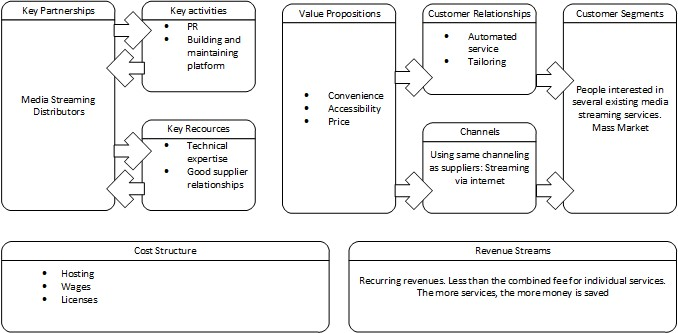
\includegraphics[scale=0.7]{./pics/model_canvas}
        \caption{The Business Model Canvas for our project}
        \label{fig:model_canvas}
    \end{center}
\end{figure}


\subsubsection*{Customer Segments}
Our product aims for an already existing market, although we want to change this market. Nonetheless, it is a mass market, consisting of people interested in several existing media streaming services.

\subsubsection*{Value Propositions}
We are focusing on the customers, who seeks several streaming services, collected in one place and at a lower price. That means there are three services of value for the customers: Convenience, accessibility and price. Convenience comes in collecting the product in one place, and making the interface painless to use. Accessibility is in the amount of suppliers, as more suppliers give wider range of streaming possibilities. Pricing lies in how far down we can push the price, which is also dependent on the suppliers, among other possibilities, such as advertisement.

\subsubsection*{Channels}
There are several ways of reaching our customers. The one way we are sure of is the fact that we want to offer our services through the same experience as existing services offer them: Streaming over the internet. It is important to note that this has to be done over several platforms, to gain competitive value through accessibility. This includes applications for mobile devices and for consoles. Advertisement of our product can be done in several ways, but the most logical way to go about this is through the suppliers. As the customers are those already using the services that our suppliers offer, the best place to advertise is through these.

\subsubsection*{Customer Relationships}
As the existing companies do, being the suppliers of our product, we want to offer an automated service through a personal profile. Through this, it is possible to offer service without greater work effort, as well as the customer being able to mend their profile to their needs. As an extra feature, we want the customer to be able to tailor their own profile to their needs. They should only have access to and pay for the services needed, in the case they only want a subset of supplier services. With personal profiles, it is possible through algorithms to use knowledge on past activity to aid the user in their experience and to suggest future actions. If a customer seems to never use the services from a specific supplier, then we can give awareness of this, such that the user can tailor the profile further.

\subsubsection*{Revenue Streams}
Through the personal profile as an automated service, we want to create earnings through subscription fees. As the most successful streaming services have their income through this method, we see no reason to change this. We want to tempt customers to use our service by being cheaper than using all the services of the customers separately. Furthermore, to tempt customers to buy more, they are given greater offers the more suppliers they add to their profile.

\subsubsection*{Key Resources}
The most important resources for this project is partnerships with the suppliers and technical expertise. If we do not have suppliers, we don't have a service. If we do not keep the suppliers satisfied with our partnership, we lose them again. Technical expertise means therefore both in our knowledge as developers, but also in public relations. The most needed resources are therefore intelligent and human resources.

\subsubsection*{Key Activities}
As the business comes up and running, the main activity is maintenance in both relationships and in customer support. If we do not continue our partnership with the suppliers, we cannot guarantee our main contribution from the service, and therefore lose customers. If the customers are unhappy with the product, we will lose them if we aren't able to locate and handle the problem.

\subsubsection*{Key Partnerships}
The media streaming distributors are our main suppliers, as they give access to the motion pictures our customers want to see. without these, the rest of the business will crumble. It is worth to note that this creates a great risk, as if we cannot live up to the expectations of our suppliers, we can lose these.

\subsubsection*{Cost Structure}
There are three major cost factors for this project: Hosting, wages and licenses. We need hardware, software locales and technical expertise for hosting. As we need expertise in some areas, such as public relations, there is a greater cost in waging. Furthermore, there is the licensing cost, as we must pay the suppliers for their service to us. We want to handle this as a percentile split, depending on the individual customer. A certain amount from each subscription is dedicated to the suppliers. The amount is based on how the customer has tailored the profile, and how much this individual is paying. Depending on what supplier services the customer has been using, the amount of money is then split, to give those that contribute to the individual customer a greater share of the profit. Another way is to make a fixed arrangement with each supplier, giving the possibility of a greater variety, and therefore a greater attraction value for new customers.